\chapter{Modelling sparse triangular solve}

\section{Analysis of sparse triangular solve} 
\label{sec:sds}

In this section we analyse the data transferred between the different cache levels
and the floating point operations performed during sparse solve which are used
as input for performance model established in the next section.
%
Therefore we analyze the different instantiations of the loops resulting from
algorithm~\ref{alg:algo:fw} and~\ref{alg:algo:bw}.
hereby we only consider on the innermost loops and do not 
distinguish between updates of~\vr{} or temporary arrays~\vtemp{}.

All coefficients of the $l$ matrix are stored as double-precision floating-point
numbers in \vlnz{}, consuming $8$\,B each. 
Elements of the \vxlnz{} (column start indices in \vlnz{}) and \vxindx{} (start
indices of row indices for each panel) arrays are stored as $8$\,B integers,
whereas for the entries of \vindx{} (row indices for each panel) $4$\,B integers
are used.

\subsection{Data transfers and FLOPs without unrolling}
\label{sec:pm:dt}
\label{sec:pm:dt:wou}

\begin{figure}[t]
  \centering
 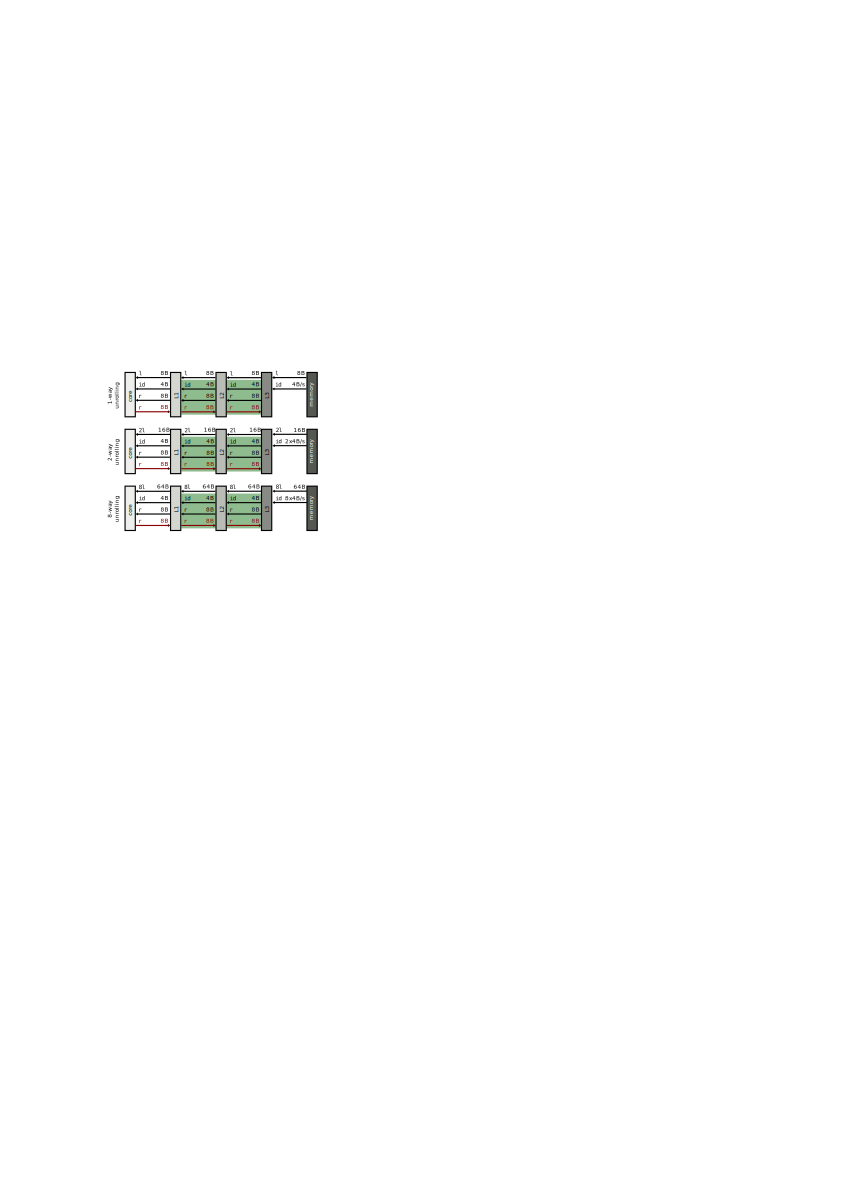
\includegraphics[width=0.43\textwidth,clip=true]{images/ecm-datatransfers}
  \caption{Data transfers for one iteration of the forward
    (including red text and arrows) and backward (without red text and arrows)
    substitution when $1$-, $2$-, or $8$-way column unrolling is applied.
    thereby $1$, $2$, or $8$ nonzero elements of \vlnz{} are processed,
    respectively.
%    loading of \vindx{} from memory (blue boxes) is only included in the model 
%    if the panel size $s \le 8$.
% from which cache level \vr{} is reused (green boxes) depends on the size of the
% active part. if the active part is large it must be reloaded from
% l3 cache. with decreasing size it can fit into l2 or even l1 cache.
% this holds also true for \vindx{}, but additionally depends on the panel size.
  }
  \label{fig:ecm:data}
\end{figure}

In the most simple case no unrolling is applied and the innermost loop of
forward substitution from algorithm~\ref{alg:algo:fw} looks like
%
\begin{algorithmic}[1]
  \setcounter{ALG@line}{22}
  \For{k = \nxlnz[j] + offset; k < \nxlnz[j+1]; ++k}
      \State row = \nindx[i++]
      \State \nr[row] -= \nr[j] \nlnz[k]
  \EndFor
\end{algorithmic}
As the loops from lines $6$--$9$ and $10$--$13$ are in principal the same as the
one in lines $23$--$26$, we only discuss the latter.
%
During each iteration one nonzero is processed, two floating point operations (FLOPs) are performed,
namely a multiplication and an addition, and the following elements get
loaded and stored, loaded: \vindx{} ($4$~\,B), \vr{} ($8$~\,B), \vlnz{}
($8$~\,B); stored: \vr{} ($8$~\,B).

How much data is transferred inside the cache hierarchy depends on the size of
the caches, their replacement strategies, the size of \vr{}, the average panel
size, as well the structure of the panels.
here we assume \vr{} is small enough to be kept at least in last level cache
(LLC) and temporal locality ensures it is not evicted.
%
Row indices in \vindx{} for a panel are loaded from memory for the panel's first
column and then are reused during each iteration over the panel's remaining
columns from the LLC in the worst case.
With panel size $\panelsize=1$, for each element of \vlnz{} one row index is
transferred and no reuse is possible.
In general reuse is only possible, starting with a panel's second column for
panel sizes $\panelsize \ge 2$.
%
Coefficients of \vlnz{} are always streamed in from memory, as they are
used only once and the \vlnz{} array is typically too large to be kept in LLC.
Figure~\ref{fig:ecm:data} visualizes the transfers assuming 
\vr{} is cached in L3 cache.

During iterating over panels and columns, the number of column elements
decrease as $l$ is a lower triangular matrix.
Thereby also the number of used elements from \vr{} decreases, which we call the
active part of \vr{}.
At some point the active part can be completely kept in L2 or even L1 cache.
this also holds true for \vindx{}, except when a new panel starts, then
the panel's row indices must first be loaded from memory.
%%
%The active part of \vr{} can be kept inside a certain cache size $c_s$, when
%concurrently also one column of \vlnz{} and the active part of \vindx{} fit into
%this cache level.
%Let $n_j$ be the length of column $j$. 
%If $l$ is dense, like for the dense matrix, then if $n_j \le c_s/(8\,\text{B} + 8\,\text{B} +
%4\,\text{B})$ holds true all active parts fit into the cache.
%%
%If instead in the worst case $l$ is sparse so that only one element out of a cache
%line from \vr{} is accessed
%then $n_j \le c_s/(8\,\text{B} + 64\,\text{B} + 4\,\text{B})$ is required.
%%
%Note that already when the active part of \vr{} slightly exceeds the determined
%limits already partial caching in the same cache level takes place\footnote{If
%we
%load a vector which exceeds the cache size several times it must be completely
%reloaded during each iteration. 
%However, if the cache utilizes a least recently used policy and the vector's
%size is in the range of the cache size $c_s$ and $c_s + w_s$, where $w_s$
%denotes the way size of the cache, then still parts of the vector are held in
%the cache and need not to be reloaded.
%The way size of a cache is defined as the product of the cache's number of sets
%and the cache line size.}.

The innermost loop of the backward substitution from
algorithm~\ref{alg:algo:bw}, looks like 
% the innermost loop from lines $5$--$9$ is the same as the one from lines
% $17$--$20$ of the backward
% substitution from algorithm~\ref{alg:algo:bw}, which we only discuss the former,
% which looks like 
%
\begin{algorithmic}[1]
\setcounter{ALG@line}{4}
  \For{k = \nxlnz[j] + offset; k < \nxlnz[j+1]; ++k}
    \State row = \nindx[i++]
    \State \nr[j] = \nr[j] - \nr[row] \nlnz[k]
  \EndFor
\end{algorithmic}
%
As this loop from lines $5$--$8$ is the same as the one from lines $17$--$20$,
all following statements hold true for both. 
%
As with forward substitution one nonzero is processed, two FLOPs are performed,
but only loads occur: \vindx{} ($4$~\,B), \vr{} ($8$~\,B), and \vlnz{} ($8$~\,B).
Note that $j$ is unchanged in the inner most loop, hence $\nr[j]$ always refers
to the same element and is not considered for the data transfer analysis.
%
Figure~\ref{fig:ecm:data} displays the data transfers occurring for one
nonzero update, if \vr{} is cached in L3 cache.

\subsection{Data transfers and FLOPs with unrolling}
\label{sec:pm:dt:wu}
%
As noted in sect.~\ref{sec:algo} it is beneficial to handle several columns
at once.
In PARDISO loops over columns are additionally to no unrolling $2$- and
$8$-times unrolled and used when a panel contains more than one column. 
With an unrolling factor of two the inner most loop for forward substitution
becomes
%
\begin{algorithmic}[1]
  \State nj = nonzero column length
  \For{k = \nxlnz[j] + offset; k < \nxlnz[j+1]; \textcolor{blue}{k += 2}}
      \State row = \nindx[i++]
      \State \nr[row] = \nr[row] - \nr[j] \nlnz[k] \textcolor{blue}{- \nr[j+1] \nlnz[k+nj]}
  \EndFor
\end{algorithmic}
%
In contrast to no unrolling per iteration two nonzeros are processed.
Hence, four FLOPs are performed and two entries of \vlnz{} are loaded.
hereby the corresponding element of \vr{} must only be loaded once instead of
twice, when processing two elements of \vlnz{}.
All other transfers stay unchanged.
%
In general with an $u$-way unrolling during each iteration $2 \times u$\,FLOPs
are executed and $u \times 8\,\text{B} + 20\,\text{B}$ are transferred.

Unrolling of the backward substitution loop results in the following code for a
two-way unrolling
%
\begin{algorithmic}[1]
  \State nj = nonzero column length
  \For{k = \nxlnz[j] + offset; k < \nxlnz[j+1]; \textcolor{blue}{k += 2}}
      \State row = \nindx[i++]
      \State \nr[j]   = \nr[j] - \nlnz[k] \nr[row]
      \State \textcolor{blue}{\nr[j+1]   = \nr[j+1] - \nlnz[k+nj] \nr[row]}
  \EndFor
\end{algorithmic}
%
Also here four FLOPs per iteration are performed, two entries of \vlnz{} are
loaded and the corresponding element of \vr{} is loaded only once.
%
For an $u$-way unrolling $2 \times u$\,FLOPs and $u \times 12\,\text{B} +
8\,\text{B}$ are loaded.

As already noted, we assume \vr{} and a panel's current row indices from
\vindx{} are at least cached in LLC or higher cache levels.
%
Unrolling hereby only saves transfers inside the cache hierarchy.
the bytes transferred between memory and LLC are left unaffected and depend only
on the panel size.
With larger panel sizes the in total less row indices \vindx{} are needed for the
whole matrix. 

\section{Extended Roofline model \todol{todo}}

\begin{table}[tp]
  \centering
  \small
  \begin{tabular}{l|ccccccccccccccccccccccccccccccccc}
  %\hline
  %\multicolumn{10}{c}{forward}  && \multicolumn{10}{c}{backward} \\
  %\cline{2-11} \cline{13-22}
  %u & l1 & \mcct{l2} & \mcct{l3} & \mcct{mem} && l1 & \mcct{l2} & \mcct{l3} & \mcct{mem}\\
  %\hline
  %1 & 14   & 4 & -- & 14  &  4 & -- & 14  & 4 & -- & 6    && 10   & 4 & -- & 10 & 4&  --&  10 & 4 & -- &6 \\ 
  %2 &  9   & 4 & -- &  9  &  4 & -- &  9  & 4 & -- & 5    &&  7   & 4 & -- &  7 & 4&  --&   7 & 4 & -- &5 \\
  %8 & 5.25 & 4 & -- & 5.25&  4 & -- & 5.25& 4 & -- & 4.25 && 4.75 & 4 & -- & 4.75&4&  --& 4.75& 4 & -- &4.25 \\
  %\hline
  \end{tabular}
  \caption{\todol{todo: add the table with Code balance}}
%  \caption{Code balance $B_c$ [B/flop] of forward/backward substitution for
%different unrollings (u) when
%data is fetched from the corresponding level inside the memory hierarchy. Values
%depend on actual panel size $s$ and possible cache reuse.}
  \label{tab:mrm:bc}
\end{table}

\todop{different section? (micro-benchmark)}
%
The attainable memory bandwidth $b$ is measured with a micro-benchmark,
ideally resembling the applications memory access pattern. 
%
The code balance $B_c$ is the ratio of by bytes transferred to the number of
floating point operations performed in the code.
In the best case, when panel size $\panelsize$ is large and the indices are
cached, during forward~\eqref{eq:algo:fw:pardiso} and backward
substitution~\eqref{eq:algo:bw:pardiso} each nonzero of $l$ must be loaded once
and the loading of indices can be neglected,
respectively. 
Furthermore the computation involves two floating point operations (FLOPs) per
nonzero.
As nonzeros are stored in double precision consuming $8$\,B, this results in a
best case code balance of $B_c = 8 / 2 \text{B/flop} = 4 \text{B/flop}$.
Table~\ref{tab:mrm:bc} lists the code balance for different unrollings and cache
levels and uses the data transfers from sect.~\ref{sec:sds}.
%
In contrast the \textit{machine balance} $B_m$ defines these ratio for the hole system
and uses the ratio of attainable memory bandwidth $B$ to maximum floating point
performance $P_\text{max}$.
This is found in table~\ref{} for all systems.
%
If $B_c > B_m$ then the code's performance is limited by the memory bandwidth,
hence it is memory bound.
This is the case for sparse direct solve for all unrollings, when data is
located in L2, L3, or memory.

To determine performance limits we only consider the case when data resides in
memory.
Hence, as fig.\ref{fig:ecm:data} indicates, only the number of nonzeros of $l$ and the
corresponding indices are relevant and is independent of the loop unrollings.
%
However we distinguish between the parallel phase, where the parts are handled,
depending on the number of threads $t$ and the serial part, where the separator
is treated, as they achieve different bandwidths as shown later, separately.
We use the following formula for a certain matrix $a$ factorized and solved with
$t$ threads:
%
\be
  p^{a}(t) 
  = \frac{
      \text{nnz} (l) \times 2 \frac { \text{flop}}{ \text{nz}}
    }{
     \frac{d_a^p(t) }{  b(t) } + \frac{ d_a^s(t) }{ b(1) }
    } \left[ \frac{\text{flop}}{s} \right],
\ee
%
where $\text{nnz}(l)$ denotes the number of nonzeros of the factor $l$ 
resulting from a factorization of $a$ for $t$ threads,
$b(t)$ is the attainable memory bandwidth with $t$ threads,
$d_a^p(t)$ the data volume of nonzeros and indices made up by the parallel 
parts, and $d_a^s(t)$ the data volume made up by the nonzeros and indices of the
separator.
%
Please note that both data volumes $d_a^p(t)$ and $d_a^s(t)$ depend on
$a$ and the number of threads $t$.
%
We extract $d_a^p(t)$ and $d_a^s(t)$ from the factorized matrices.
%

% all coefficients of the $l$ matrix are stored as double-precision floating-point
% numbers in \vlnz{}, consuming $8$\,b (byte) each. 
% elements of the \vxlnz{} and \vxindx{} arrays are stored as $8$\,b
% integers, whereas for the entries of \vindx{} $4$\,b integers are used.
% 
% during forward~\eqref{eq:algo:fw:pardiso} and backward
% substitution~\eqref{eq:algo:bw:pardiso} each nonzero of $l$ must be loaded once, 
% respectively. 
% further the computation involves two floating point operations (flops).
% in the best case the panel size $\panelsize$ is large and the indices are cached, hence
% they must only be loaded once for the panel from memory.
% this case has a \textit{code balance}, the ratio of transferred bytes between
% memory and cpu compared to the number of flops performed, of $b_c = 8/2$ b/flop
% $= 4$~b/flop.
% this is clearly higher than the machine balance $b_m$ in table~\ref{tab:hw} of all
% evaluated systems, which indicates that the code is memory-bound.
% 
% for performance prediction $p_\text{rfm}^a(t)$ we model the parallel phase,
% where the parts are handled and the serial part, where the separator is treated
% separately.
% we use the following formula for a certain matrix $a$ solved with $t$ threads:
% %
% \be
%   p_\text{rfm}^{a}(t) 
%   = \frac{
%       \text{nnz} (l) \times 2 \frac { \text{flop}}{ \text{nz}}
%     }{
%      \frac{d_p^a(t) }{  b(t) } + \frac{ d_s^a(t) }{ b(1) }
%     } \left[ \frac{\text{flop}}{s} \right],
% \ee
% %
% where $\text{nnz}(l)$ denotes the number of nonzeros of the factor $l$ from $a$
% \todo{depends this on the number of threads?},
% $b(t)$ is the attainable memory bandwidth with $t$ threads,
% $d_p^a(t)$ the data volume of nonzeros and indices made up by the parallel 
% parts, and $d_s^a(t)$ the data volume made up by the nonzeros and indices of the
% separator.
% please note that for the data volumes $d_p^a(t)$ and $d_s^a(t)$ depend both on
% $a$ and also on the number of threads $t$.
% we extracted the data volumes $d_p^a(t)$ and $d_s^a(t)$ from the factorized
% matrices.
% also note that possible loop unrolling (discussed later in
% section~\ref{sec:pm:dt:wu}) has no impact on the transferred data volume between
% cpu and memory here.

The attainable memory bandwidth depends on the access pattern of the
application.
Hence, it is crucial to choose a benchmark for measuring which resembles the
application's behavior for more precise predictions.
In case of sparse direct solve this is a read only benchmark where only one
vector is read from memory. 
%
Typically memory bandwidth benchmarks utilize vectorized loads and stores.
However, sparse solve in PARDISO only uses scalar instructions as it is not
vectroized by the compiler.
\todol{likwid-bench, different section}

% if enough cores are used then scalar and vectorized benchmarks saturate the
% memory bandwidth with the only difference that the saturation of the latter
% is already achieved with less cores. this is shown in figure~\ref{fig:mrm:bw-scaling} 
% exemplified on the hsw1 and hsw2 system.
% %
% as for our modified roofline model also the single core bandwidth is relevant we
% use for all bandwidth measurements the scalar read only benchmark.
% figure~\ref{fig:mrm:bw-single-core} shows the difference between the scalar and
% vectorized versions for the single core and the full processor or cluster for
% all systems in the test bed (except sx).
% 
% \begin{figure}[tp]
%   \centering
%   \subfloat[]{%
%     \includegraphics[height=0.3\textheight,clip=true]{images/stream/streamreadhswscalarvectorized}
%     \label{fig:mrm:bw-scaling}
%   } \,
%   \subfloat[]{%
%     \includegraphics[height=0.3\textheight,clip=true]{images/stream/streamreadsinglecorefullprocessor}
%     \label{fig:mrm:bw-single-core}
%   }
%   \caption{bandwidth over the number of cores of the read only benchmark in a
% scalar and vectorized version exemplified on hsw-d and
% hsw-s~\protect\subref{fig:mrm:bw-scaling}.
% single core bandwidth and saturated bandwidth with all available cores of the
% processor/cluster~\protect\subref{fig:mrm:bw-single-core}.}
%   \label{fig:mrm:bw}
% \end{figure}

%\section{ECM model}